\newpage
\section{第 7 课}

\subsection{脑图}

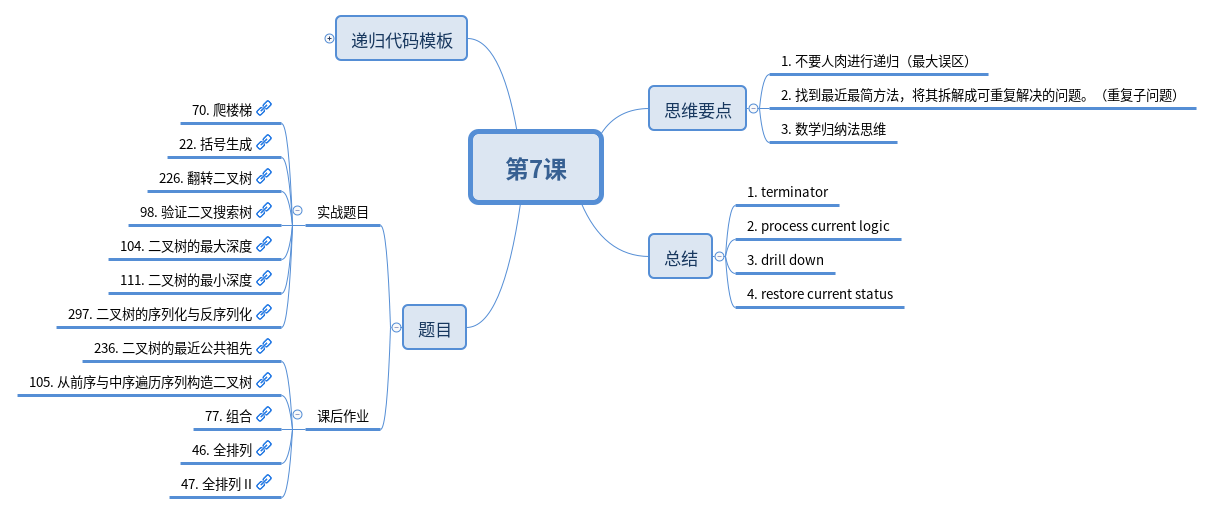
\includegraphics[width=170mm,height=80mm]{images/第7课.png}

\subsection{题目}

\subsubsection{实战题目}

\begin{itemize}
  \item \hyperref[leetcode:70]{70. 爬楼梯}
  \item \hyperref[leetcode:22]{22. 括号生成}
  \item \hyperref[leetcode:226]{226. 翻转二叉树}
  \item \hyperref[leetcode:98]{98. 验证二叉搜索树}
  \item \hyperref[leetcode:104]{104. 二叉树的最大深度}
  \item \hyperref[leetcode:111]{111. 二叉树的最小深度}
  \item \hyperref[leetcode:297]{297. 二叉树的序列化与反序列化}
\end{itemize}

\subsubsection{课后作业}

\begin{itemize}
  \item \hyperref[leetcode:236]{236. 二叉树的最近公共祖先}
  \item \hyperref[leetcode:105]{105. 从前序与中序遍历序列构造二叉树}
  \item \hyperref[leetcode:77]{77. 组合}
  \item \hyperref[leetcode:46]{46. 全排列}
  \item \hyperref[leetcode:47]{47. 全排列 II}
\end{itemize}
